\capitulo{5}{Aspectos relevantes del desarrollo del proyecto}
%%%%%%%%%%%%%%%%%%%%%%%%%%%%%%%%%%%%%%%%%% Borrar
\begin{comment}
Este apartado pretende recoger los aspectos más interesantes del desarrollo del proyecto, comentados por los autores del mismo.
Debe incluir desde la exposición del ciclo de vida utilizado, hasta los detalles de mayor relevancia de las fases de análisis, diseño e implementación.
Se busca que no sea una mera operación de copiar y pegar diagramas y extractos del código fuente, sino que realmente se justifiquen los caminos de solución que se han tomado, especialmente aquellos que no sean triviales.
Puede ser el lugar más adecuado para documentar los aspectos más interesantes del diseño y de la implementación, con un mayor hincapié en aspectos tales como el tipo de arquitectura elegido, los índices de las tablas de la base de datos, normalización y desnormalización, distribución en ficheros3, reglas de negocio dentro de las bases de datos (EDVHV GH GDWRV DFWLYDV), aspectos de desarrollo relacionados con el WWW...
Este apartado, debe convertirse en el resumen de la experiencia práctica del proyecto, y por sí mismo justifica que la memoria se convierta en un documento útil, fuente de referencia para los autores, los tutores y futuros alumnos.

\end{comment}
%%%%%%%%%%%%%%%%%%%%%%%%%%%%%%%%%%%%%%%%%% COMIENZO

En este punto se recogerán los aspectos más relevantes del desarrollo comentando en cada caso las decisiones tomadas para llegar a nuestros objetivos haciendo un resumen de la experiencia práctica del proyecto, de cómo se solucionaron los problemas encontrados en cada caso y la relevancia que tuvieron en el alcance total del proyecto.

\section{Motivación del proyecto}
El proyecto se me ocurrió hace años cuando me emancipé a una vivienda con las persianas motorizadas que me parecieron que podrían hacer una función mayor si dispusieran de cierto equipamiento, y cogió fuerza con la llegada de la pandemia de la COVID19 cuando el tema surgió en distintas conversaciones en las que que había quien no podía acercarse a sus segundas viviendas y estaban preocupados por una posible ocupación. Tras darle vueltas a esta situación surgió la idea de crear un sistema domótico para poder ayudar a quien lo precise con este proyecto.

\section{Formación necesaria}
El proyecto requirió muchas horas de búsqueda de ideas por la web, ya que no existe información fiable de cómo realizar una instalación de estas características sino que existen muchos pequeños proyectos amateur que se centran en cubrir una pequeña necesidad; siendo proyectos que no disponen de un respaldo documental detrás. Abundan las soluciones de profesionales de otros campos que quieren probar a hacer sus propias soluciones de carácter amateur.

Por ello, para poder desarrollar el proyecto me vi en la necesidad de visitar numerosas páginas web de distinta índole para hacerme a la idea de cómo podría enfocar el proyecto. Aunque, el mayor hándicap a la hora de realizar este proyecto es la desinformación, por lo que me apoyé sobre todo en el REBT~\ref{concepto:RETB}~\cite{manual:REBT} y en mis conocimientos básicos de motores fruto de formación pasada.

La información de cómo funcionan los GPIO la obtuve tras realizar el curso de: “Control de GPIO con Python en Raspberry Pi” de Programo Ergo Sum~\cite{misc:programoergosum}.
Aunque parte la información de la web de <<bujarra>>~\cite{misc:BujarraGPIO} está desactualizada, esta publicación me ayudó a comprender cuál era el funcionamiento real de un relé y cómo conectarlo a los GPIO.

Otro punto importante a la hora de enfocar correctamente el proyecto fue el estudio del REBT~\cite{manual:REBT}, de su apartado BT-21~\cite{manual:ICT-BT-21}, del reglamento de ICT~\cite{manual:ICT} y los estándares de comunicaciones como son el IEEE802.11~\cite{manual:IEEE802.11} y el TIA568~\cite{manual:568.1}~\cite{manual:568.2}. Creo necesario confrontar estas normativas para poder realizar un proyecto a nivel profesional y documentalmente respaldado.

\section{Metodología}
Se eligió Scrum como la metodología global sobre la que realizar el proyecto de forma iterativa y ágil. Buscamos generar un proyecto lo más cercano a cómo sería un proyecto de este tipo en el ámbito laboral, pero salvando las distancias con un grupo de trabajo real con el que poder interactuar. Aunque he tenido reuniones semanales con los tutores no se ha realizado un seguimiento diario pero sí se cumplieron, en cualquier caso, unas reglas generales mínimas:

\begin{itemize}
    \item Los trabajos se desarrollaron en forma de <<sprints>> semanales.
    \item Tras cada <<sprint>> semanal se realiza una entrega de trabajo de forma incremental.
    \item En cada revisión del <<sprint>> se disponen los trabajos a realizar durante la semana.
    \item Realizando una revisión semanal, el proyecto goza de flexibilidad al integrar cambios sobre trabajos pequeños de forma que el proyecto está en constante mejora.
    \item Sobre el Kanban se realiza la estimación de tiempos por tareas según dificultad.
    \item Se priorizan las tareas del proyecto según mayor valor de negocio.
    \item Se cambia el estado de los <<issues>>, mediante un Kanban, según evoluciona el trabajo.
    \item Comprobamos como avanza el proyecto con los gráficos BurnDown de que dispone Zenhub.
\end{itemize}

Reseñar que en las fases de trabajos físicos no se ha aplicado Scrum pero se ha realizado con un criterio lo más cercano posible. Por ello, se predispuso realizar la tirada de cable y el conexionado la misma semana para que pudiera integrarse lo mejor posible en la metodología.

\section{Desarrollo del proyecto}
A medida que el proyecto ha ido tomando forma también se han ido implementando cambios: La idea original del proyecto era parametrizar los elementos según horas pero posteriormente se valoró e implantó la idea de tomar datos externos para poder controlar los elementos del sistema domótico. El proyecto se ha creado de forma cronológica siguiendo los pasos que se desarrollan a continuación.

El proyecto se comenzó por los scripts de extracción de datos para comprobar que se podía realizar el software que se había propuesto antes de continuar ya que es más fácil presentar cambios al principio que cuando el proyecto está avanzado. Aunque cabe destacar que se ha invertido una gran cantidad de tiempo en la búsqueda de información y normativas que desconocía, así como en la extracción y el tratamiento de datos.

Por tanto, se comenzó extrayendo datos desde Python~\cite{misc:Python} mediante web scraping (es una forma de recopilar información de páginas web) pero nos dimos cuenta de que una web es más susceptible de sufrir cambios. Por ello, recurrimos a APIS de terceros sin coste para poder realizar dicha extracción de datos, y tratándolos como json~\cite{misc:Json} extraer los datos que nos interesen.

\subsection{Extracción de datos}
Los algoritmos de extracción y tratamiento de datos también han ido cambiando ya que se han ido modificando las APIS para obtener más datos y de carácter más fiable.

Al comenzar a extraer datos de la API de geolocalización de~\url{www.ifconfig.me/ip} me obtenía la ubicación de la provincia, lo cual no es nada exacto ya que tendremos temperaturas diferentes según ubicación. Por ello, me vi obligado a hacer una búsqueda más a fondo para encontrar una API que se ajustase a las necesidades del proyecto. Tardé algunos días hasta que encontré \url{http://ip-api.com} que me entregaba más información y más fiable. Además, en el mismo intervalo, pasamos de utilizar web scraping a tratar los datos directamente como json~\cite{misc:Json}, que también es un cambio importante.

\begin{figure}
    \centering
    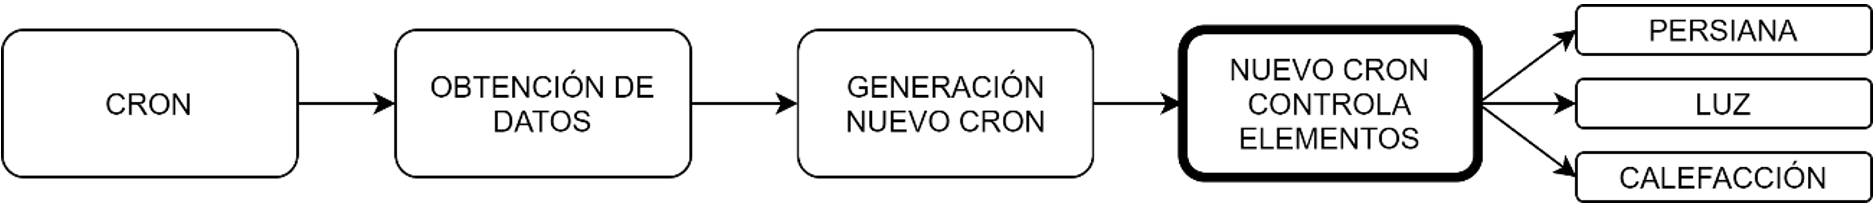
\includegraphics[width=\textwidth]{img/Cron1.PNG}
    \caption{Proceso de obtención de datos, programación de tareas y ejecución.} \label{Img:Cron1}
\end{figure}

En la segunda API, en el caso de~\url{www.weatherapi.com} podía obtener únicamente los valores de salida y puesta de sol para realizar el control de las persianas pero también era insuficiente, por lo que tuve que volver a hacer una búsqueda más amplia hasta que encontré~\url{www.climacell.co}, que me entrega las temperaturas de las próximas horas además de otros muchos parámetros que pueden llegar a servirnos como, por ejemplo, la velocidad del viento o si será un día nublado.

Tras obtener la ubicación de la instalación y extraer los parámetros necesarios de las APIS pasamos a conformar el archivo de datos para generar la configuración de Cron (Cron, es el programador de tareas de Linux~\cite{misc:Linux}). Podemos ver el contenido del archivo que se genera en el sistema para poder trabajar con él en el~\ref{lst:Ejemplo}. Esta fase dispone de varios pasos:

\begin{enumerate}
    \item Desde <<Cron>> se llama al script de toma de datos.
    \item Conformamos el nuevo archivo de <<Cron>>.
    \item El nuevo <<Cron>> lanza los scripts según las horas predispuestas.
\end{enumerate}

De esta manera el control de los dispositivos se hará automáticamente desde <<Cron>> con los datos actualizados diariamente. Podemos ver un diagrama explicativo de este proceso en la imagen~\ref{Img:Cron1}. Además, podemos ver a continuación un ejemplo de archivo de recopilación de datos:

\begin{minipage}{\linewidth}
\begin{lstlisting}[language=json, basicstyle=\small, caption={Ejemplo archivo de recopilado de datos.}, label={lst:Ejemplo}]
{
"Planeta":
	{
	"Amanecer": "08:37:00",
	"Anochecer": "17:57:00"
	},

"temperaturas":
	{
	"0": 5.26,
	"1": 5.78,
	"2": 5.93,
	"3": 5.95,
	"4": 5.97,
	   ...
	"23": 2.91
	}
}
\end{lstlisting}
\end{minipage}



Este archivo de datos es leído siempre que queremos modificar alguno de los parámetros de automatización desde el bot, como son la temperatura o la hora más temprana a la que pueden bajar las persianas, además de cuando se regenera el Cron.

\subsection{Scripts}
Utilizaremos dos tipos de scripts, Bash~\cite{misc:Linux} y Python~\cite{misc:Python}.

Una vez determinados los datos que vamos a necesitar en un notebook de Jupyter debemos realizar la extracción de estas líneas de código a un script Python.
En este punto tuve un problema bastante sencillo de resolver: el script necesita importar librerías para hacerlo correr y necesitaba instalarlas. En principio, esto no debería ser un problema ya que sabemos que se puede instalar con Pip. El problema surge al tener instalado Python v2 y Python v3, ya que si instalas las librerías utilizando Pip no funcionarán con Python3. Así que, hay que instalarlas con Pip3 para poder utilizarlas desde Python3:
\begin{lstlisting}[language=sh,firstnumber=1]
pip3 install paquete
\end{lstlisting}

Controlaremos la Raspberry Pi y sus periféricos mediante comandos Bash y realizaremos el procesado de datos con Python. Se ha tomado esta determinación para conseguir la mayor velocidad de procesamiento posible así como para evitar posibles problemas. Por ello, la automatización que haremos desde CRON que lanzará otros scripts será mediante bash. 

El script que lanza todo el código contiene las siguientes líneas de código~\ref{cod:LanzaProceso}:

\begin{lstlisting}[language=sh, caption={Script que lanza el proceso automático completo.}, label={cod:LanzaProceso}]
#!/bin/bash
path=$(pwd)
echo $path

# Este script se ha desarrollado para lanzar todo el proceso desde CRON.
python3 ${path%}/1_recabaInfo.py
python3 ${path%}/3_cocinado.py
sh ${path%}/4_reescribeCron.sh
\end{lstlisting}

Este archivo es un archivo Bash porque desde Cron no he conseguido lanzar los scripts Python, sin embargo no he tenido problemas al lanzarlo desde este script Bash siempre que especifique nuevamente que se lance con python3.

Por otro lado, para controlar los relés desde los GPIO, debemos configurarlos como OUT y con valor 1 para activarlos y, con valor 0 y configuración IN para desactivarlos. Podemos ver un ejemplo a continuación, el las líneas de código~\ref{cod:reles}:
\begin{lstlisting}[language=sh, caption={Ejemplo activación y desactivación de relé.}, label{cod:reles}]
gpio -g mode 17 out # Activa el rele conectado al pin 17
sleep 1             # Espera 1 segundo
gpio -g mode 17 in  # Desactiva el relé conectado al pin 17
\end{lstlisting}

Este código lo lanzaremos tanto desde el bot directamente para controlar las persianas <<en vivo>>, como desde el Cron para el control de persianas y otros periféricos.

\subsection{Instalación física}
Quizás, la parte más compleja del proyecto ha sido la instalación física dado mi grado de desconocimiento así como el encontrar las piezas idóneas para el domicilio.

Al comienzo del proyecto, hubo una gran parte de investigación e instalación del sistema ya que quería realizar el proyecto de la forma más profesional posible. Por ello, me dispuse a bucar en el REBT~\cite{manual:REBT} y en la normativa de ICT~\cite{manual:ICT-BT-21} para no saltarme ningún paso y que la instalación fuera totalmente legal.

\begin{figure}[h]
    \centering
    \includegraphics[width=1.0\textwidth]{img/Diagrama Básico.pdf}
    \caption{Diagrama físico. } \label{Img:diagramaBasico}
\end{figure}

Fue complejo leer tanto y comprender cómo realizar los cálculos de los cables dentro de los tubos y conseguir discernir entre la asignación real entre los diferentes canales de la vivienda. Una vez comprobado que utilizaría la norma actualizada de 2020 del REBT, realicé los cálculos para comprobar que podía `tirar' el cable UTP por estos canales con seguridad. 

\begin{figure}[h]
    \centering
    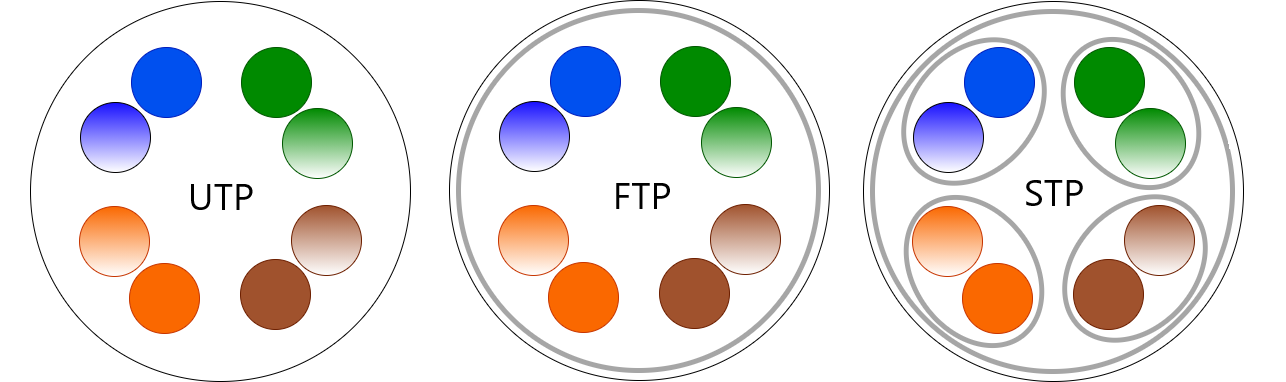
\includegraphics[width=0.9\textwidth]{img/CABLES.png}
    \caption{Disposición interna cables UTP, FTP y STP.} \label{Img:CablesDatos}
\end{figure}

En la imagen~\ref{Img:diagramaBasico} podemos diferenciar varios elementos: Por un lado, tenemos el cuadro eléctrico y la primera caja de derivación, que ya vienen instaladas en el domicilio en la misma disposición que podemos ver en el diagrama (la caja de derivación encima del cuadro eléctrico), y en medio, me dispuesto la Raspberry Pi, para que puedan llegar los cables de datos fácilmente, ya que los hemos dispuesto por los canales eléctricos hasta los diferentes elementos a controlar (persianas, luz y calefacción).

Cabe destacar una particularidad de mi instalación: el router está albergado dentro del RTR ya que sobra espacio dentro del mismo y mi router está optimizado para no calentarse en espacios con poca ventilación. El canal que podemos ver entre el cuadro eléctrico general y el RTR es una toma eléctrica que, por normativa debe estar ahí y es la que alimenta algún dispositivo que deba estar dentro de esta situación.

Estuve valorando la opción de ‘tirar’ un cable de datos desde la primera caja de derivación después del Cuadro General de Mando y Protección o Cuadro eléctrico, hasta el RTR (Registro Terminación de Red) que es donde tengo la línea de datos más cercana, pero en único canal que comunica es de naturaleza eléctrica y no está bien mezclar tipos de instalaciones.


Buscando por Internet he podido ver que es más sencillo utilizar medios inalámbricos ya que no tendríamos que hacer tirada de cable, pero no me ofrecen la misma garantía ante un posible fallo de comunicación o interferencias, y con el cable eliminamos la posibilidad de sufrir este tipo de problemas. Sobre la categoría del cable, me he decantado por UTP cat5e (Ver imagen~\ref{Img:CablesDatos}) porque es un cable suficientemente capaz de transmitir los 3.3V en pico de nuestra Raspberry Pi y el precio no es muy alto.


\subsection{Pruebas Físicas}

\begin{figure}[h]
    \centering
    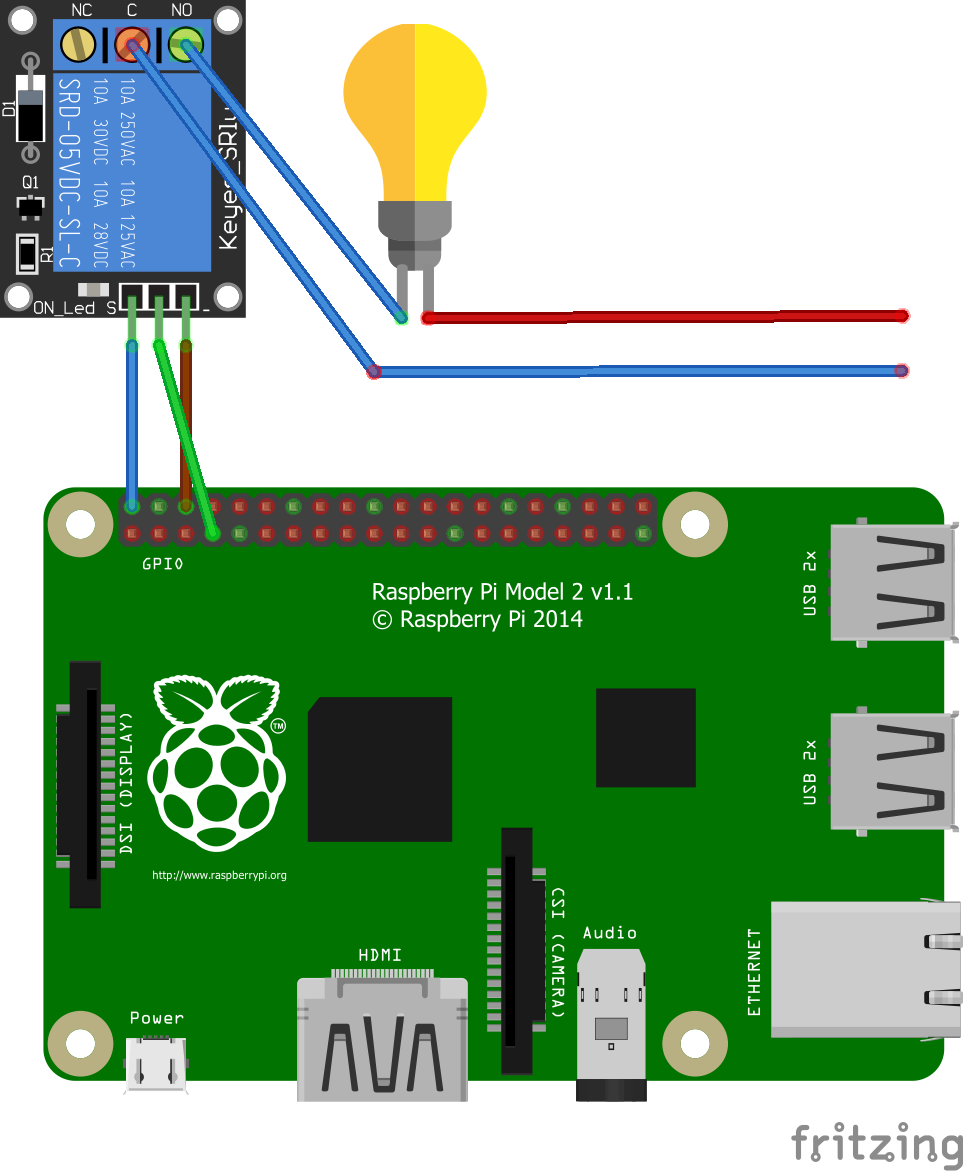
\includegraphics[width=0.6\textwidth]{img/Plano_Placa_Pruebas.png}
    \caption{Plano de tablero de pruebas.} \label{Img:Plano_Placa_Pruebas}
\end{figure}

La primera prueba, consistía en la instalación de la Raspberry Pi con un relé (ver imagen~\ref{Img:Rele1}) y una bombilla conectada a 220VAC (VAC:Voltage Alternating Current), y se llevó a cabo con éxito. Podemos ver un diagrama de como se conectó en la imagen~\ref{Img:Plano_Placa_Pruebas}.

Llegados a este punto, era interesante el comprobar que se podía lanzar correctamente un script de este tipo desde CRON, encendiendo y apagando la bombilla, que también fue un éxito.

La tirada de cable y conectorizado en todo el domicilio, desde la primera caja de empalmes a las 5 persianas ya que es el punto del domicilio donde se recogen los cables eléctricos que llegan hasta las persianas, quedó como podemos ver en el diagrama~\ref{Img:diagramaBasico}. 
\subsection{Telegram Bot}\label{5.TelegramBot}
En primer lugar, explicaré qué es un bot. El medio de comunicación con el sistema domótico es un bot de Telegram que he diseñado y programado para hacer completamente funcional el proyecto. Desde el Bot, podemos controlar las persianas de forma instantánea, modificar la configuración del sistema domótico y simulador de presencia, volver a generar recolección de datos y el grabado de los archivos. También podemos obtener información sobre la información recopilada, sobre nuestra Raspberry Pi y sobre el funcionamiento futuro del sistema domótico y simulador de presencia.
\begin{figure}
    \centering
    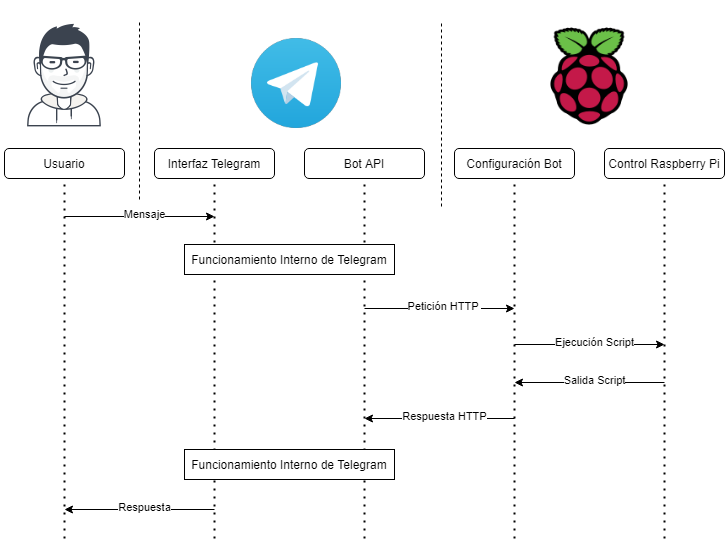
\includegraphics[width=0.95\textwidth]{img/Diagramas/FuncionamientoBot.png}
    \caption{Comunicación del bot. } \label{Img:FuncionamientoBot}
\end{figure}


Afortunadamente estaba mejor documentado que el resto de la recursos que he consultado para el proyecto pero aún así no ha resultado tarea fácil entender la lógica del bot. 
Podemos ver la lógica de comunicaciones del bot en la imagen~\ref{Img:FuncionamientoBot}. 

Todos los mensajes de Telegram que llegan a nuestro bot, tienen la misma estructura json, pero de esta estructura utilizamos únicamente unos pocos y podríamos resumir en los que figuran en las líneas de código~\ref{lst:Resumen}, y que podemos ver a continuación:
\begin{lstlisting}[language=json,firstnumber=0, basicstyle=\small, caption={Resumen de los datos que utilizamos del mensaje de Telegram.},label={lst:Resumen}]
{
    'content_type':'text',
    'message_id':0000,
    'text':'a',
    'chat':{
        'id':000000000,
        'first_name':'David',
        'last_name':'David',
        'username':'David'}
}
\end{lstlisting}

Al comienzo del proyecto pensé en crear un grupo de usuarios para gestionar esta información pero he creído oportuno que cada usuario tenga su propia interfaz aunque realmente no habría problema en hacerlo de esta manera y hubiera facilitado el proyecto. Esto se ha solucionado incluyendo la lista de usuarios que pueden interactuar con el bot en el archivo de configuración. Para este paso, debemos recoger el id del usuario. Este id aparece varias veces en el json que recibimos en cada mensaje por lo que valdría cualquiera de ellos. Para el resumen he escogido el id que pertenece al objeto chat, junto al nombre y apellidos del propietario y el nombre de usuario.
El número de usuario es necesario para saber a quién le enviamos el mensaje. Por ejemplo, al comienzo del bot del proyecto tenemos las siguientes líneas del código~\ref{cod:mensajeInicio}:

\begin{lstlisting}[language=Python, caption={Código para el envío de mensajes al inicio del bot.}, label={cod:mensajeInicio}]
for usuario in usuarios:
    bot.send_message(usuario, "Iniciando Sistema a las "+str(hora))
\end{lstlisting}

Estas líneas envían un mensaje de inicio con la hora a la que se produce el evento a cada uno de los usuarios de la lista de admitidos.

Otro de los puntos necesarios es el de texto que envía el usuario. Gracias a éste obtendremos la orden que enviamos por Telegram y podremos actuar en consecuencia.
Hay un punto a tener en cuenta para comprender el funcionamiento del bot, éste radica en las líneas que hay al principio de cada uno de los métodos de que dispone el bot, y que podemos ver en las líneas de código~\ref{cod:llamadas}:

\begin{lstlisting}[language=Python, caption={Código de llamada a funciones desde el bot.}, label={cod:llamadas}]
@bot.message_handler(commands=['temp'])
@bot.message_handler(func=lambda message: message.text == "t")
@bot.message_handler(func=lambda message: message.text == "T")
def command_long_text(m):
    usuario = m.chat.id
    if (compruebaUsuario(m)):
        temperaturasManana.temperaturas(m , bot)
\end{lstlisting}

En ellas podemos ver, por orden, el comando temp, al que podemos acceder enviando el comando \texttt{/temp}. Posteriormente vemos dos funciones lambda, éstas significan que si introducimos únicamente esa letra también lanzará el método. He introducido estos comandos rápidos para facilitar la introducción de órdenes.
Observamos que si el usuario que escribe está en la lista de admitidos, lanzará el método temperaturas pasándole el mensaje enviado y el objeto bot, que contiene información sobre el usuario y el mensaje que envía.
Por último, el método al que se llama, recoge esta información y opera en consecuencia según lo que se le pida, bien con una función u otro método.